\uuid{pfqd}
\exo7id{7118}
\titre{exo7 7118}
\auteur{megy}
\organisation{exo7}
\datecreate{2017-02-08}
\isIndication{true}
\isCorrection{true}
\chapitre{Géométrie affine euclidienne}
\sousChapitre{Géométrie affine euclidienne du plan}
\module{Géométrie}
\niveau{L2}
\difficulte{}

\contenu{
\texte{
% n'utilise que des triangles isocèles et rectangles
Soit $\mathcal C$ un cercle de centre $O$, $[AB]$ une corde et $\mathcal T$ la tangente de $A$. Alors $(\mathcal T,AB)=\frac12(OA,OB)$.

\begin{center}
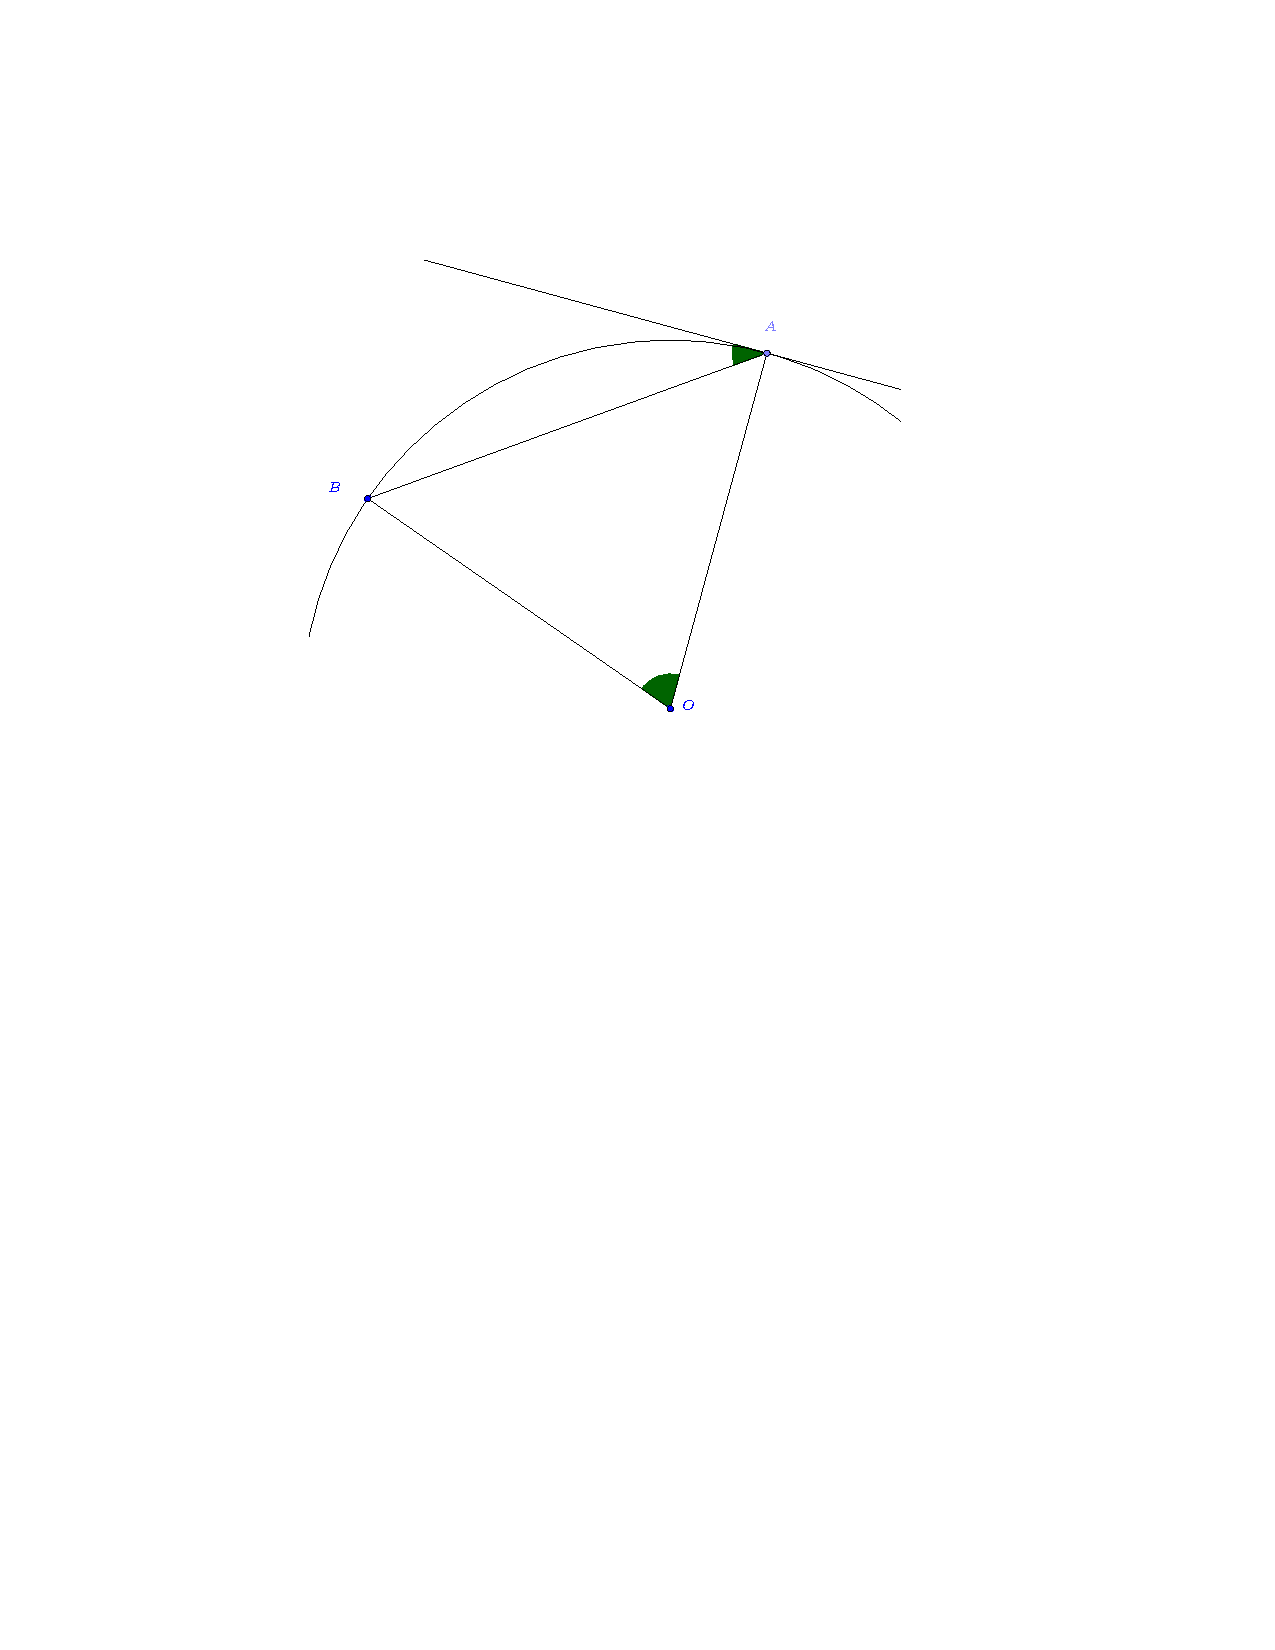
\includegraphics{../images/img007118-1}
\end{center}
}
\indication{Triangles isocèles et rectangles}
\reponse{
Traçons la figure, où on a placé $I$ le milieu de $[AB]$, de telle sorte que $\frac12(OA,OB)=(OA,OI)$.

\begin{center}
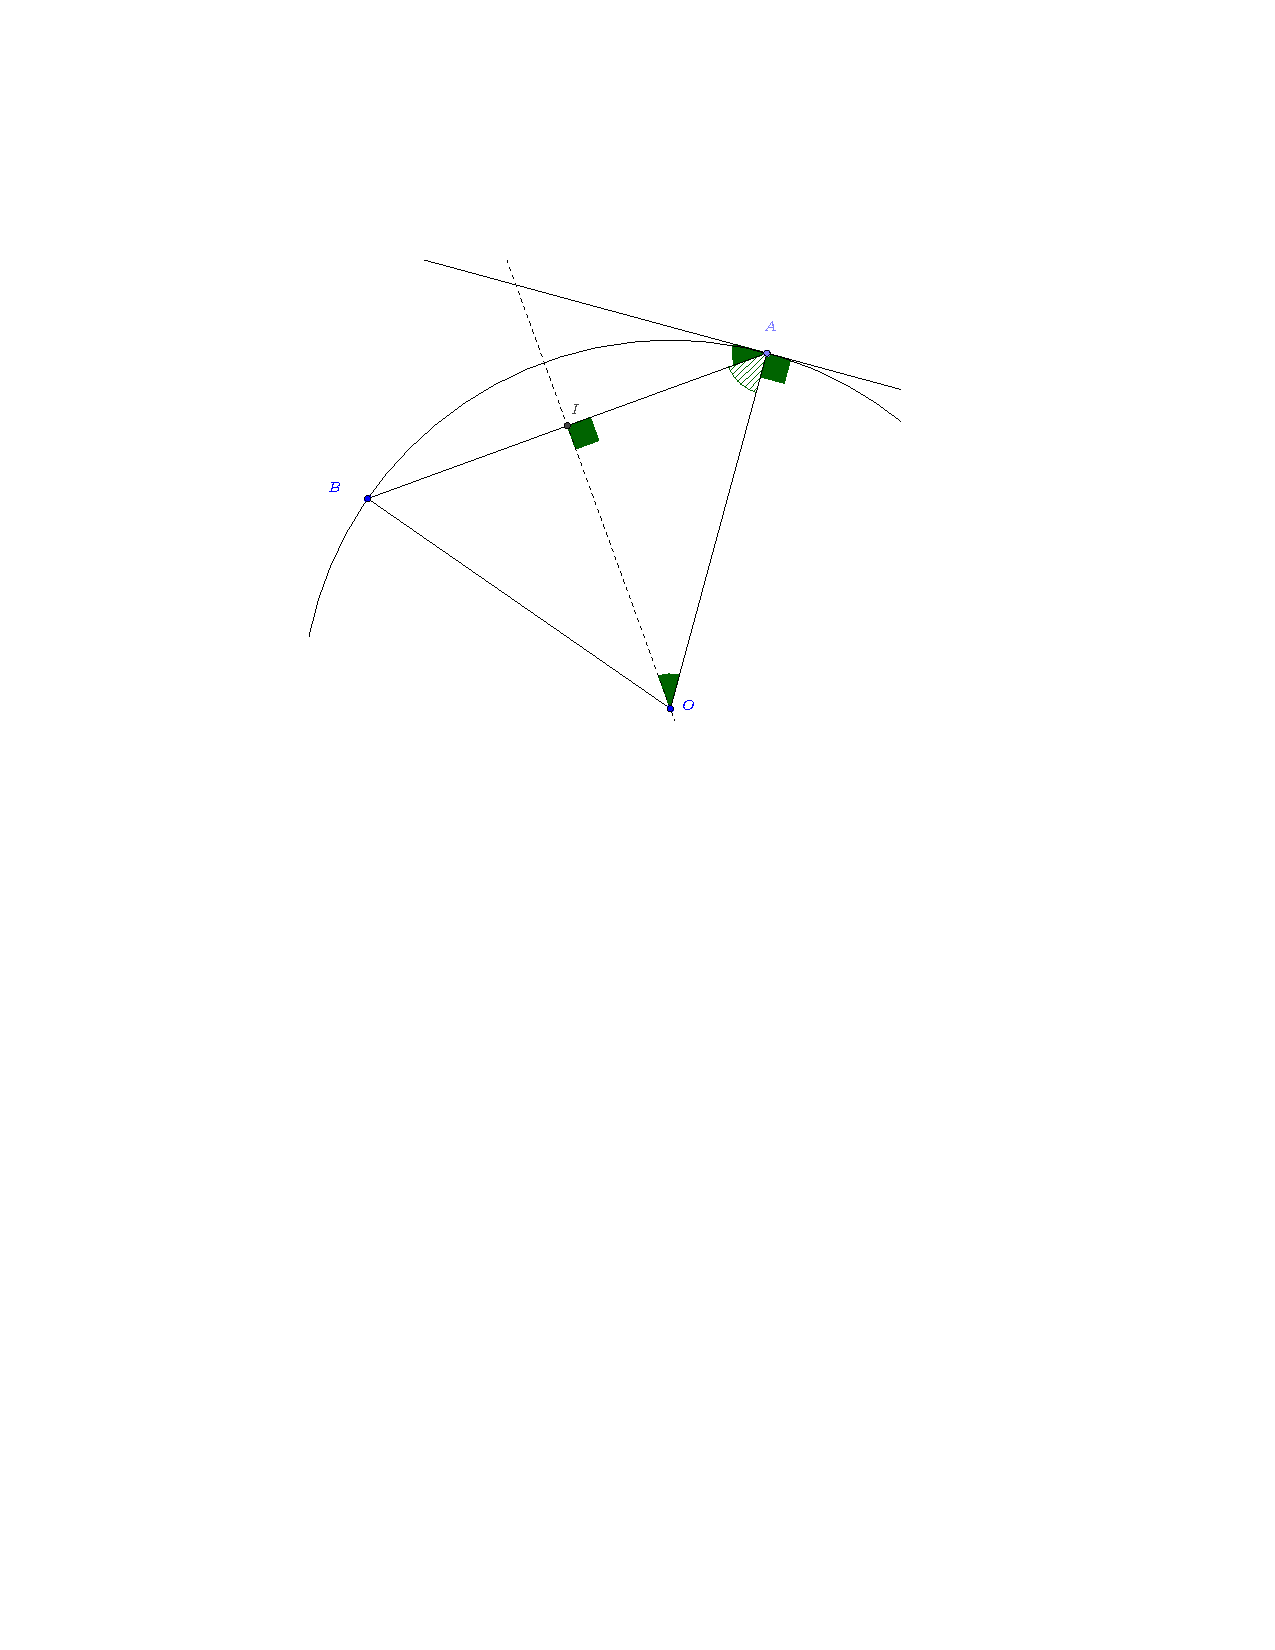
\includegraphics{../images/img007118-2}
\end{center}


Les angles $(AO,\mathcal T)$ et $(AI,IO)$ sont droits.
On a d'une part :
\[ 0=(\mathcal T,\mathcal T) =  (\mathcal T,AI) +(AI,AO)+ \pi/2, \]
et d'autre part, dans le triangle $AIO$:
\[ 0=(AI,AO)+(IO,IA)+(OA,OI)=(AI,AO)+\pi/2+(OA,OI).\]
Finalement, on a donc:
\[ (\mathcal T,AB) = (\mathcal T, AI) = -(AI,AO)-\pi/2 = (OA,OI)=\frac{1}{2}(OA,OB),\]
ce qu'il fallait démontrer.$\qed$
}
}
